\chapter[Positionsregelung]{Verifizierung der Positionsregelung der ETH-Z�rich in Verbindung mit einem Laserscanner}
\label{chap:Positionsregelung}

In einer Zusammenarbeit von \gls{asctec} und der ETH-Z�rich wurde eine Regler zur Positionierung des Pelican Quadrocopters in geschlossenen R�umen entworfen und ver�ffentlicht. Der Entwurf basierte dabei auf einer monokularen Kamera �ber die mittels eines \gls{vslam}-Algorithmus und der Fusion der \gls{imu} die Position des Flugobjekts in der unbekannten Umgebung ermittelt wird. Regelung- und Fusionsalgortihmus sind im Paper \cite{Achtelik11} beschrieben. Aufgabe dieses Kapitel ist es die dort ver�ffentlichen Annahmen und Formel zu verifizieren. Dies erfolgt �ber Literaturrecherchen und Herleitung der publizierten Gleichungen. Unter Ber�cksichtigung, das die Position nun mehr vom Laser �ber die Kapitel \ref{chap:2Dpositionsbestimmung} vorgestellten Algortihmen bestimmt wird, ist Abschnitt \ref{sec:strukpositionsregelung} darauf ausgelegt eine �bersicht �ber die Bestandteile der Regelung zu geben. Herleitung der Komponenten erfolgt in den anschlie�end Unterkapiteln. 

\section{Struktur der Positionsregelung}
\label{sec:strukpositionsregelung}
Das Hauptaugenmerk diese Unterkapitel liegt darauf, wie sich die Positionsregelung in die in Kapitel \ref{sec:Kommunikationsarchitekur} vorgestellte Systemstruktur einf�gt. Welche Softwarekomponenten daf�r auf dem \gls{hlp} integriert wurden. Wie die Kommunikation zwischen ihnen und der Umgebung aussieht. Mit dem Ziel ein grundlegendes Verst�ndnis f�r die Funktionsweise der Regelung zu generieren.\\
\begin{figure}
	\centering
	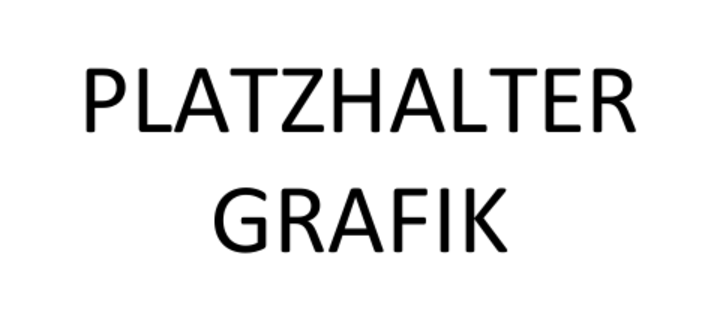
\includegraphics[width = .55\textwidth]{images/Platzhalter}
	\caption[Kaskadenstruktur]{Reduzierte Kaskadenstruktur der Positonsregelung. } %
	\label{fig:kaskstruc}
\end{figure}


Die Positionsregelung wird auf die Lageregelung (engl. Attitudecontrol) aufgesetzt. Daraus resultiert eine Kaskadenstruktur (Abbildung \ref{fig:kaskstruc}). Diese Vorgehensweise ist nachvollziehbar, da die Lageregelung bereits Fest auf dem \gls{llp} implementiert ist. Diese besteht aus einem Regelalgorithmus der anhand der Regeldifferenz der Orientierung $e_{ori}$, resultierend aus der Abweichung Soll-Orientierung $O_s$ und Ist-Orientierung $ O  $, in Verbindung mit der Sollschubvorgabe $ T_s $ die Drehzahlen $ n_{1..4} $ der Rotoren berechnet und einstellt. Die Ist-Orientierung $ O =\begin{bmatrix} \phi&\theta&\psi\end{bmatrix}^T $ wird mittels eines Fusionsfilter bestimmt. Dieser fusioniert die Messwerte der auf der \gls{imu} befindlichen Gyroscope mit den Daten des 3D-Kompass. Wie dieser unterlagerte Regler und der dazugeh�rige Zustandssch�tzer genau ausgef�hrt sind ist nicht bekannt. Eine m�gliche Ausf�hrung ist in Paper \cite{hoffmann10} beschrieben. Die Ungewissheit �ber den Regleraufbau der Lageregelung stellt f�r den Entwurf der �berlagerten Positionsregelung kein Problem dar. Von Interesse ist lediglich, das die Annahme einer sehr hohen Dynamik des Reglers zur einer Vereinfachung des f�r die Positionsregelung ben�tigen Modells (Kapitel \ref{sec:Modelbildung}) f�hrt. Hohe Dynamik bedeutet, das der die Sollwinkel in einer sehr kurzen Zeit $ t \rightarrow 0~s $ erreicht wird. 

 
\begin{figure}
	\centering
	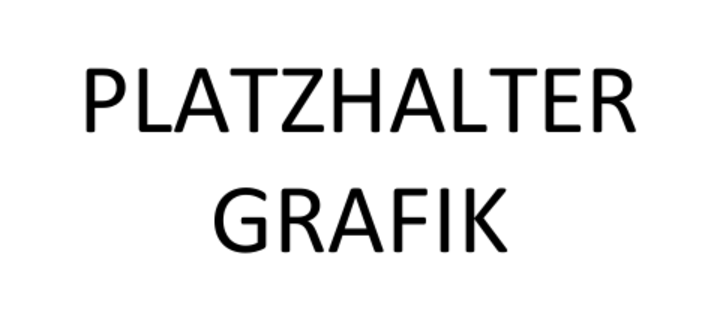
\includegraphics[width = .55\textwidth]{images/Platzhalter}
	\caption[Gesamtstruktur Regelung]{Struktur der Regelung} %
	\label{fig:strucregelung}
\end{figure}


\section{Modellbildung}
\label{sec:Modelbildung}